\documentclass[oneside]{tum-book}

\title{Proposal to Bachelor's thesis}
\subtitle{Auto-generation of business process models using natural language processing}
\author{Shuaiwei Yu}
\matnr{03741718}

\chair{Chair of Information Systems and Business Process Management (i17)}
\school{TUM School of Computation, Information and Technology}
\department{Department of Computer Science}
\degree{Bachelor of Science}

\examiner{Prof. Dr. Stefanie Rinderle-Ma}
\supervisor{Catherine Sai, M. Sc.}

\hood{Garching}
\submissiondate{15.04.2023}

\begin{document}
  \chapter*{Abstract}
\noindent
Business Process Modeling Notation, also known as BPMN, is a vital tool that provides a structured and understandable visualization of the company's workflow. Leveraging such techniques can positively impact the company's workflow execution and improvement. However, generating BPMN models requires domain-specified knowledge and is often time-consuming, yet adopting approaches that automatically identify and extracts process models can prominently minimize the time and effort of process modelling.

Natural Language Processing (NLP) is a discipline that developed rapidly in recent years, which is an interdisciplinary discipline focusing on the study of algorithms that enable the computer to understand and process the human languag. With credit to NLP technology, researchers can now develop tools that analyze the business process descriptions and develop tools to perform automatic extraction of relevant BPMN information.

Based on the state-of-art BPMN model generation algorithms, this article rebuilds the program with a more recent technique using \textit{python} and an open-source library \textit{spacy} as well as improves the recognition accuracy.



\textit{\textbf{Keywords: }BPMN, NLP, LLM, machine learning}

  \newpage

  \tableofcontents
  \listoftables
  \listoffigures
  \newpage

%inkscape for visulization

  \chapter{Motivation}

%	bpmn introduce
	Business processes are fundamental elements for companies and organizations. They aggregate all the tasks, activities, and timelines involved in companies' workflow whose aim is to provide business or to create value \cite{literature_review_2}. Business Process Modeling Notation, also known as BPMN is a modeling language describing such workflows by using graphical notations and thus provides an easily understandable overview of the operations performed in the organization for all business users \cite{literature_review_1}. 
	
	Due to the importance of Business processes, leveraging the BPMN techniques can positively affect an organization's performance and thus increase its productivity. However, not everyone is familiar with the BPMN designing techniques. Consequently, managers, along with other process participants prefer using natural language to define business processes. As a result, organizations usually have a large amount of information stored as text documents \cite{literature_review_2}. There is a need to translate text documents into the process model regarding such a situation. However, process modeling is not a simple task, but is time-consuming and experts with professional knowledge are required. 
%todo: if there is a need to expand the details of difficulties of process modeling, then refer to literature_review_2 
	
%	nlp introduce
	Over the past years, the development of AI techniques brought solutions to many technical difficulties. Natural Language Processing (NLP), as one of the AI's branches, could possibly address the problem of the difficulties in process modeling. Natural Language Processing is an interdisciplinary discipline focusing on the study of algorithms that enable the computer to understand and process the human language\cite{t2m_3}. During the understanding and processing of the natural language text, NLP performs three types of analysis: Firstly, morphological analysis is performed, which analyze the structure of words. The syntactic analysis then explores the grammar relationship between words in sentences, deciding which grammar category the word belongs to. Finally, semantic analysis is executed, which leverages the afore analyses to define the meaning of the text based on the knowledge of sentence structure and the relationship between words \cite{literature_review_2}. 
%todo: if there is a need to expand the details of NLP analysis, then refer to literature_review_2 introduction part
	
%	why should nlp be used to generate the bpmn
	The unique features of the NLP technique make it very suitable for exploiting information from the text documents that record the firm's business process and then analyzing the data to generate the process models automatically. This paper serves as a proposal to suggest using NLP to extract the information from text written in nature language and automatically generate the corresponding business model.
	
	\section{Research Questions}

	The main research question (\textbf{RQ}) is formulated as: "\textit{How can business process models be generated from regulatory documents automatically using the Nature language processing technique?}". To better answer the main research question, three embedded aspects can be revealed: \textbf{RQ1}: "\textit{which NLP methods can be used to extract information?}"; \textbf{RQ2}: "\textit{How can the extracted information be analyzed and composed to generate business process models?}" and finally \textbf{RQ3}: "\textit{How does the proposed approach perform with different kinds of input documents?}"

	
	Currently, there exist various tools, libraries, and dependencies for NLP. Therefore, the first research question \textbf{RQ1} tries to figure out which methods are the most suitable ones to use to extract information from regulatory documents. The methods should be able to separate sentences, label each word in a sentence with corresponding syntactical tags, and analyze the grammatical relationships between words. By doing so, we are able to explore the information hidden behind the natural language and thus use them for further operation. In the next step, \textbf{RQ2} explores how to use syntactical and grammatical information to determine events of business processes, identify the conditional restraints ("and" or "or"), and the sequential orders of business processes. Once such information is acquired, an algorithm should be developed to combine all the business processes in a logical order. In the end, the composed process model should be well visualized. The last research question \textbf{RQ3} tries to discover the adaptability of the proposed model: How well does the method perform with the document other than the regulatory document? Does the accuracy of the outcome decrease with other kinds of documents? A sets of different input documents will be prepared and a corresponding benchmark will be performed. 
  \chapter{Research Methodology}

Design science is a paradigm of real-world problem-solving by creating innovative artifacts. Therefore, Design science research tightly connected the IT artifact with the application domain. Furthermore, the need and desire to improve the current environment and methods motivate Design science research and therefore requires innovative artifacts to address such problems \cite{DSM_1}. We adopted the research methodology of \cite{DSM_2} here and followed the research process model given in their work.

\section{Problem centered approach}
Although some work in the current field was done, we wanted to develop better tools to automatically extract the business process model for the broad audience of end users, i.e., users within a business organization with little knowledge about business process modeling or underlying technologies. Such motivation provides us with an opportunity to work on creating the tool mentioned above. This problem-centered approach leads us to the first step of the research process, according to \cite{DSM_2}.

\section{Problem Identification And Motivation}
Modeling business processes requires experts with relevant knowledge and can be exhausting and time-consuming. Thus, small companies usually cannot afford such experts and business managers usually prefer to describe processes using natural language. As a result, an organization usually process a large amount of text documents  \cite{literature_review_2}. However, the business process provides an intuitional overview of the business process and can potentially increase a company's productivity.

\section{Objectives of a solution}
Our objective is to create an easy-to-use tool that uses the Nature language processing technology to automatically extract information from organizations' regulatory documents and generate business process models.

\section{Design \& development}
The development of the new artifact adopted the critical success chain (CSC) method, which uses literature to support and consolidate the conceptual basis of the artifact designing \cite{DSM_2}. We addressed the issues and the needs identified earlier, such as how to find a proper tool to extract information from regulatory documents or how to process such information to generate a BPMN model. We conducted a literature review and used the helpful information from the selected papers to combine their ideas and develop our own artifact. The intended artifact is to develop a prototype that leverages the NLP technique to automatically extract business process models from regulatory documents.

\section{Demonstration}
In the demonstration activity, we want to illustrate how we can use our new artifact to solve instances of problem \cite{DSM_3}. We plan to implement a web-based front-end so that customers can use our artifact rather easily, even if they have no knowledge of programming. The customer can enter the textual description which is a regulatory document into an input field on the website and click a button to send the request to convert the text to the BPMN model. Then the regulatory document will be sent to the backend and processed there. Finally, the customer will be able to see a BPMN model presented in an image on the website.

\section{Evaluation}
The evaluation phase is vital in the design of an artifact. The evaluation examines how well the designed artifact solves the problem, which involves comparing the the actual output of the problem and the output generated by the artifact \cite{DSM_3}. We intended to first manually generate business process models using several different kinds of documents. Then we will use our artifact with the same documents  




The evaluation measures how well the artifact supports a solution to the problem. This activity involves comparing the objectives of a solution to actual observed results from use of the artifact in context. Depending on the nature of the problem venue and the artifact, evaluation could take many forms. At the end of this activity the researchers can decide whether to iterate back to step three to try to improve the effectiveness of the artifact or to continue on to communication and leave further improvement to subsequent projects.



\section{Communication}
To ensure the delivery of the desired artifact, every aspect of the problem and the design of the artifact will be communicated and discussed with the relevant stakeholders \cite{DSM_3}. Since this is a bachelor's thesis, the primary contact is the author's advisor. Furthermore, we will also seek advice and suggestions from Prof. Dr. Stefanie Rinderle-Ma and the corresponding Chair of Information Systems and Business Process Management (i17).







  \chapter{Related Work}

	In order to learn the current state-of-the-art methods of auto-generating business process models and thus answer the research question comprehensively, a systematic literature review must be performed so that what kind of efforts are made can be learned as well as what are the most preferred techniques and what open challenges exist. The literature review is conducted under the guidance of Kitchenham et al. given in their paper \cite{literature_review_guidance}. The work consists of several stages: Firstly, the electronic database used to run the search is chosen. Then the selection criteria are defined, and articles are filtered accordingly. After that, a horizontal search will be run to cover as many papers as possible. Finally, a list of the final literature is studied carefully, and helpful information is extracted.
	
% search string
	To perform a comprehensive literature review, three most famous electronic databases are chosen, i.e., IEEE, Springer, and ACM. Nevertheless, only using these three databases, There is still a minor chance that some important articles will be missed. Therefore, Google scholar was also used as a complement because it covers a wide range of literature, from conference papers to degree theses. The search string used for the literature review is developed using two phrases, which are the most important ones for our research: \textit{business process model} and \textit{natural language processing}.
	
% selection criteria
	In the next step, inclusion and exclusion criteria should be defined. They describe a list of desired and undesired features for the literature selection to obtain relevant studies and support our research and future work. Inclusion criteria were developed as follows: \textbf{IC-1}: NLP should have high relevance to the research paper. \textbf{IC-2}: BPMN should have high relevance to the research paper. \textbf{IC-3}: The research paper should describe the generation of the BPMN model using NLP. Exclusion criteria were: \textbf {EC-1}: the research paper is not written in English. \textbf{EC-2}: The research paper is not in the form of a proper scientific article. 
	
		\begin{table}[]
		\begin{center}
		\caption{\centering Overview of Systematic Literature Review Protocol}
		\begin{tabular}{lccl}
    	\textbf{Database}\hspace{30mm} & \textbf{hits} & \textbf{selected} &  \\
    	\hline
		IEEE                     		& 56   & 5   &      		\\
		Springer                 		& 275  & 8   &      		\\
		ACM                      		& 201  & 2   &      		\\
		Google scholar           		& 31   & 3   &      		\\
		\hline
		Result horizontal search	 	& 563  & 18  &      		\\
		Vertical search          		&      & 4   &  \hspace{5mm}add papers  \\
		\hline
		Overall                  		&      & 22   &     
		\end{tabular}
		\end{center}
		\floatfoot{number of hits using the search string in different databases.}
	\end{table}
	
	During the literature selection, the first step was to identify duplicates since multiple electronic databases were used. Duplicates refer to articles that have the same title and authors. In the next step, the article's title, abstract and introduction parts were read and the inclusion and exclusion criteria were applied to shape the final result further. Finally, the whole article was read and then a vertical search was performed to identify the related papers used in our selected papers. As a final result, 17 papers were chosen. 
	
	Among the chosen papers, \cite{literature_review_1} \cite{literature_review_2} \cite{literature_review_3} \cite{literature_review_4} are literature reviews that analyzed the development and usage of process model generation methods. \cite{literature_review_3} points out that the NLP is the most widely adopted method and it can also be combined with other methods to increase accuracy. \cite{literature_review_1} and \cite{literature_review_3} give a list of tools for NLP and process model generation that have been used in previous works. \cite{literature_review_4} compares several papers using NLP to extract process models with different inputs and concludes the typical steps that have to be performed. \cite{complement_2} and \cite{complement_3} propose their findings in identifying the inconsistencies between the textual description and the generated process model. \cite{complement_4} however proposed a new part-of-speech tagging method that is specifically trained for business process management, which can effectively reduce the error rate in grammatical tagging.
	
	A novel breakthrough is made in the work of \cite{t2m_1}, where a method was developed which extracts information from textual descriptions to automatically generate the business process models regardless of the structure of the input text. The paper gives an excellent overview of the steps that should be executed during the process model extraction and the potential challenge one might encounter. The Authors performed three vital steps to process the text input: (i) syntax parsing using the part-of-speech tagging method, (ii) semantic analysis using FrameNet and WordNet, and (iii) anaphora resolution. Finally, they can generate a process model based on the data. Nevertheless, their work was published in 2012, and some of the techniques could already be outdated. We see great potential here to work on an updated approach to improve the results of this work based on the paper.
	
	 Some limitations of \cite{t2m_1} are also addressed in \cite{pre_processing_1}: The textual description must be grammatically correct, otherwise the model will produce an incorrect output. Furthermore, the process in the description must develop sequentially and cannot contain examples or questions. Another work offered in \cite{t2m_2} focuses on the extraction of declarative process models to address the problem that many NLP models can only handle the imperative process models. This is done by introducing many grammatical constraints to analyze the relationship of words. This idea illustrates us to also expand the analysis of the semantic analysis so that our model is also able to deal with the textual documents that have a complex description of the process. 
	 
%	 Among all works, little effort is made to visualize the process model, \cite{complement_1} introduces a web-based NLP model extraction service. However, this work leverages the extraction model of others, and thus the output accuracy cannot be well guaranteed. As mentioned, our model should assist people who do not have a technical background in the process model generation. \cite{complement_1} gives us an idea of additionally implementing a web-based frontend that can ease the use of our tool.

% todo: what is the difference between normal text and legal (regulatory) documents: Jurix, Coliee, caise	
	
	
	
	
  \chapter{Method/Approach (theoretical)}
\label{sec:method}

  \chapter{Application (practical)}
\label{sec:application}

  \chapter{Evaluation}
  \chapter{Time Plan}

The period for the entire project is five months. Suppose our thesis begins on the 15th. April, then the submission deadline is the 15th. September. To ensure the delivery of the project with good quality, a time plan should be developed to arrange the tasks that should be performed during these five months. The tasks should be distributed fairly within the project period so that the tasks can be accomplished with caution and precision.

The tasks for the projects can be divided into several parts: \textbf{(I)} Pre-processing of the input documents, where the input documents are separated into sentences, and the part-of-speech tagging is performed. \textbf{(II)} Information extraction, where we will focus on extracting information from the sentences. This part is significant work for the whole approach. During this step, the active/passive voice issue will be addressed; the anaphora problem will be solved; the conditional markers will be detected; and all other necessary steps will be performed in this step. \textbf{(III)} Flow generation, where each business activity's interactions are identified and connected. \textbf{(IV)} Post-processing, where we use the flows to generate a BPMN model and convert it into images. \textbf{(V)} Frontend design, where we implement a front end and connect it with our backend. \textbf{(VI)} Evaluation and redesign, where we evaluate our approach and make improvements regarding the identified limitations of our approach.

\begin{figure}[h]
    \centering
    \caption{Gantt chart of project implementation}
    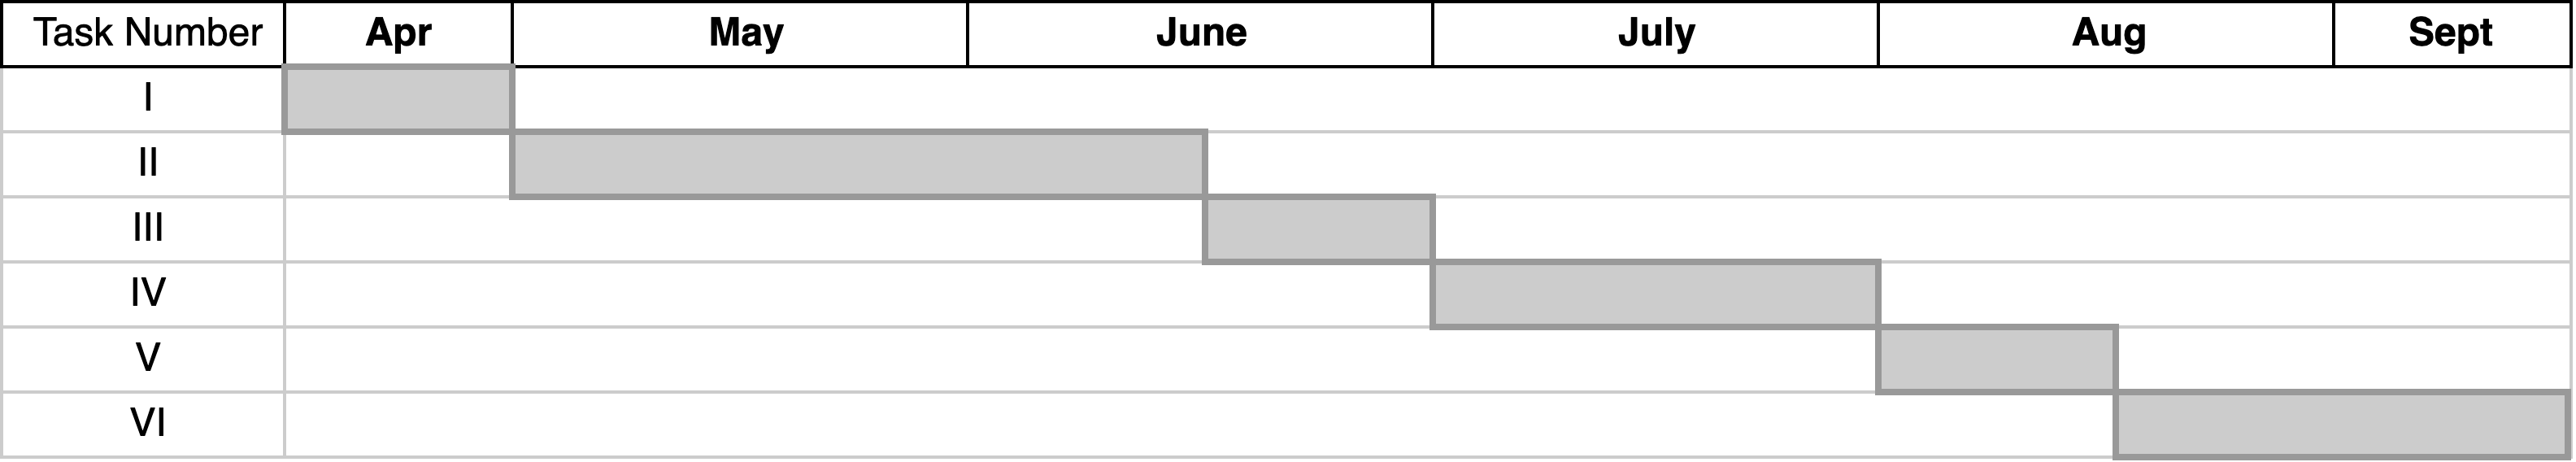
\includegraphics[width=1\textwidth]{tum-resources/images/time_plan.png}
\end{figure}

  \newpage  
  \printbibliography[heading=bibintoc]
%  \newpage
%  \chapter{Appendix}

%\begin{table}[h!]
%  \begin{center}
%    \caption{Your first table}
%    \begin{tabular}{l|c|r} % <-- Alignments: 1st column left, 2nd middle and 3rd right, with vertical lines in between
%      \textbf{Value 1} & \textbf{Value 2} & \textbf{Value 3}\\
%      $\alpha$ & $\beta$ & $\gamma$ \\
%      \hline
%      1 & 1110.1 & a\\
%      2 & 10.1 & b\\
%      3 & 23.113231 & c\\
%    \end{tabular}
%  \end{center}
%  \floatfoot{A note describing the table.}
%\end{table}

	\begin{table}[]
		\centering
		\caption{\centering Overview of Systematic Literature Review Protocol}
		\begin{tabular}{lccl}
    	\textbf{Database}\hspace{30mm} & \textbf{hits} & \textbf{selected} &  \\
    	\hline
		IEEE                     		& 56   & 5   &      		\\
		Springer                 		& 275  & 8   &      		\\
		ACM                      		& 201  & 2   &      		\\
		Google scholar           		& 31   & 3   &      		\\
		\hline
		Result horizontal search	 	& 563  & 18  &      		\\
		Vertical search          		&      & 2   &  \hspace{5mm}add papers  \\
		\hline
		Overall                  		&      & 20   &     
		\end{tabular}
	\end{table}

\newpage

\begin{figure}[h]
    \centering
    \caption{My Figure Caption}
    
\includegraphics[width=0.7\textwidth]{tum-resources/images/Universitaet_Flaggen.jpg}
    \floatfoot{A note describing the figure}
\end{figure}

\end{document}
